% !TEX root       = ./type_name.tex
% !TEX program    = pdflatex
% !TEX encoding   = utf-8
% !TeX spellcheck = en_GB
%=======================================================================

\chapter{Introduction}\label{ch:introduction}
\sffamily{}
The penetration of mobile internet users has increased many fold from a few thousands to millions over a short span of time. Due to the increasing demand for data among subscribers, mobile operators are pushed to go beyond boundaries to provide efficient and reliable data service to their customers. Although, the existing network services such as UMTS and LTE can handle larger data capacity, their coverage is not always sufficient in crowded places such as office buildings, convention centers, shopping malls etc. There is an urgent need to find a solution on how to offload the mobile data traffic over to other radio standards.

In such case, WLAN is an existing radio standard that has already been deployed in large numbers and has been supported by millions of devices lately. One unique advantage of using WLAN over other radio standards would be its license free usage of its radio frequency for commercial purposes. This WLAN standard, when deployed in a controlled manner can support data traffic routed from the mobile services. The IEEE 802.11 WLAN has already been widely used for commercial enterprises ranging from office networks, shopping malls to educational institutions etc. The deployment rages from a few dozens to hundreds of access points (APs), which serve many users through multitude of devices ranging from mobile devices, laptops to printers and other connected hardware. These networks also provide varied set of services that includes authentication, authorization and accounting (AAA), dynamic channel reconfiguration, interference management, security such as intrusion detection and prevention and providing quality of service. 

These enterprise WLAN AP’s are usually centrally managed through a controller. The task now is to find a solution to seamlessly direct traffic between LTE and WLAN. The research project BIC-IRAP (Business Indoor Coverage Integrated Radio Access Point) is currently aimed at providing a solution for the seamless coupling between LTE and WLAN.

The growing adoption of Software Defined Networking in the recent years has given rise to providing unique solutions without depending too much on hardware. The advantage of using SDN is that, it separates the network control pane from the physical network topology and uses software control flow to define how traffic is forwarded in the network. For example, the routing table and the flow control of a switch can be easily controlled remotely through a software controller.  The capabilities of SDN is possible due to the use of OpenFlow protocol which is a standardized protocol that is used by the SDN based controller to manipulate the flow tables of network switches. This provides more flexibility to programmatically control the behavior of network switches by building network applications that talk to the network controller. Any OpenFlow enabled switch from any vendor provides a common interface to be manipulated via a controller, thus providing flexibility and simplified network management.

%\comment{
%The cloud is a big deal for given reasons:
%\begin{itemize}
%	\item It does not need any effort on the consumer or the end user's part to maintain or manage it.
%	\item Any authenticated user can access the cloud-based applications and services from anywhere. All that the user needs is a device with an Internet connection.
%	\item It is effectively infinite in size, so that the consumer or the end user doesn't need to worry about it running out of capacity.
%	\item The resources can be scaled up or down quickly and easily to meet the desired changing demands of the consumer.
%	\item The services offered in the cloud are metered services, so the end user pay only for what they use.
%\end{itemize}
%}

\section{Contribution}\label{sec:contribution}

This thesis provides a novel approach towards separating the data traffic between the different network providers within an access point. This is made possible through the simple, yet effective use of OpenFlow protocol that enables the development of different enterprise WLAN services as applications such as, using software defined network controllers. The performance benefits achieved though this system is possible without any changes to the existing 802.11 client. The proposed system is compatible with the existing enterprise WLAN security protocols like WPA2 enterprise.
%\begin{itemize}
%	\item to run "in the cloud";
%	\item to be accessed over the Internet from a web browser;
%	\item to be used by large numbers of customers simultaneously at low cost.
%\end{itemize}

\section{Results}\label{sec:Results}
The expected outcome of this thesis is to demonstrate a prototype system that runs an AP on an OpenFLow controlled switch. The AP also provides enterprise grade authentication system WPA2 enterprise alongside a RADIUS server, and host two separate networks. The separation of data traffic between the two networks will take place within the same AP and provide Hotspot 2.0 functionality.

\section{Research Context\cite{BIC:IRAP}}\label{sec:BIC-IRAP}
The research described in this thesis was done based on the BIC-IRAP project which is focused on combining the strengths of LTE and Wireless-LAN seamlessly. Through the integration of small and micro cells of LTE with WLAN in the BIC-IRAP system, the two radio technologies are available through a single dynamically configurable hardware configuration.

\section{Thesis Structure}\label{sec:Structure}
This thesis report is organized as follows, Chapter 2 describes the background for this thesis. Chapter 3 describes in detail about SDN and the different types in use today. Chapter 4 talks about the control and authentication mechanism such as the protocols and technologies used. Chapter 5 talks about the environment required to build the system such as the tools and software’s. Chapter 6 describes in detail how the application is developed, from conceptualization to coding in python. Chapter 7 shows how the system is being implemented. Chapter 8 presents the results obtained from the system after series of testing and enhancement. Chapter 9 concludes the thesis and describes further improvements and drawbacks of this method.

%\begin{itemize}
%	\item \textbf{Software as a Service (SaaS)}
%	\item \textbf{Platform as a Service (PaaS)}
%	\item \textbf{and Infrastructure as a Service (IaaS)}
%\end{itemize}


%\begin{itemize}
%	\item Private cloud: with a cloud network accessible by limited and restricted permission to only particular organisation.
%	\item Public cloud: with a cloud network accessible to the general public.
%	\item and Hybrid cloud: which is partly private and secured, and partly public and accessible.
%\end{itemize}

%\begin{figure}[H]
%	\begin{center}
%		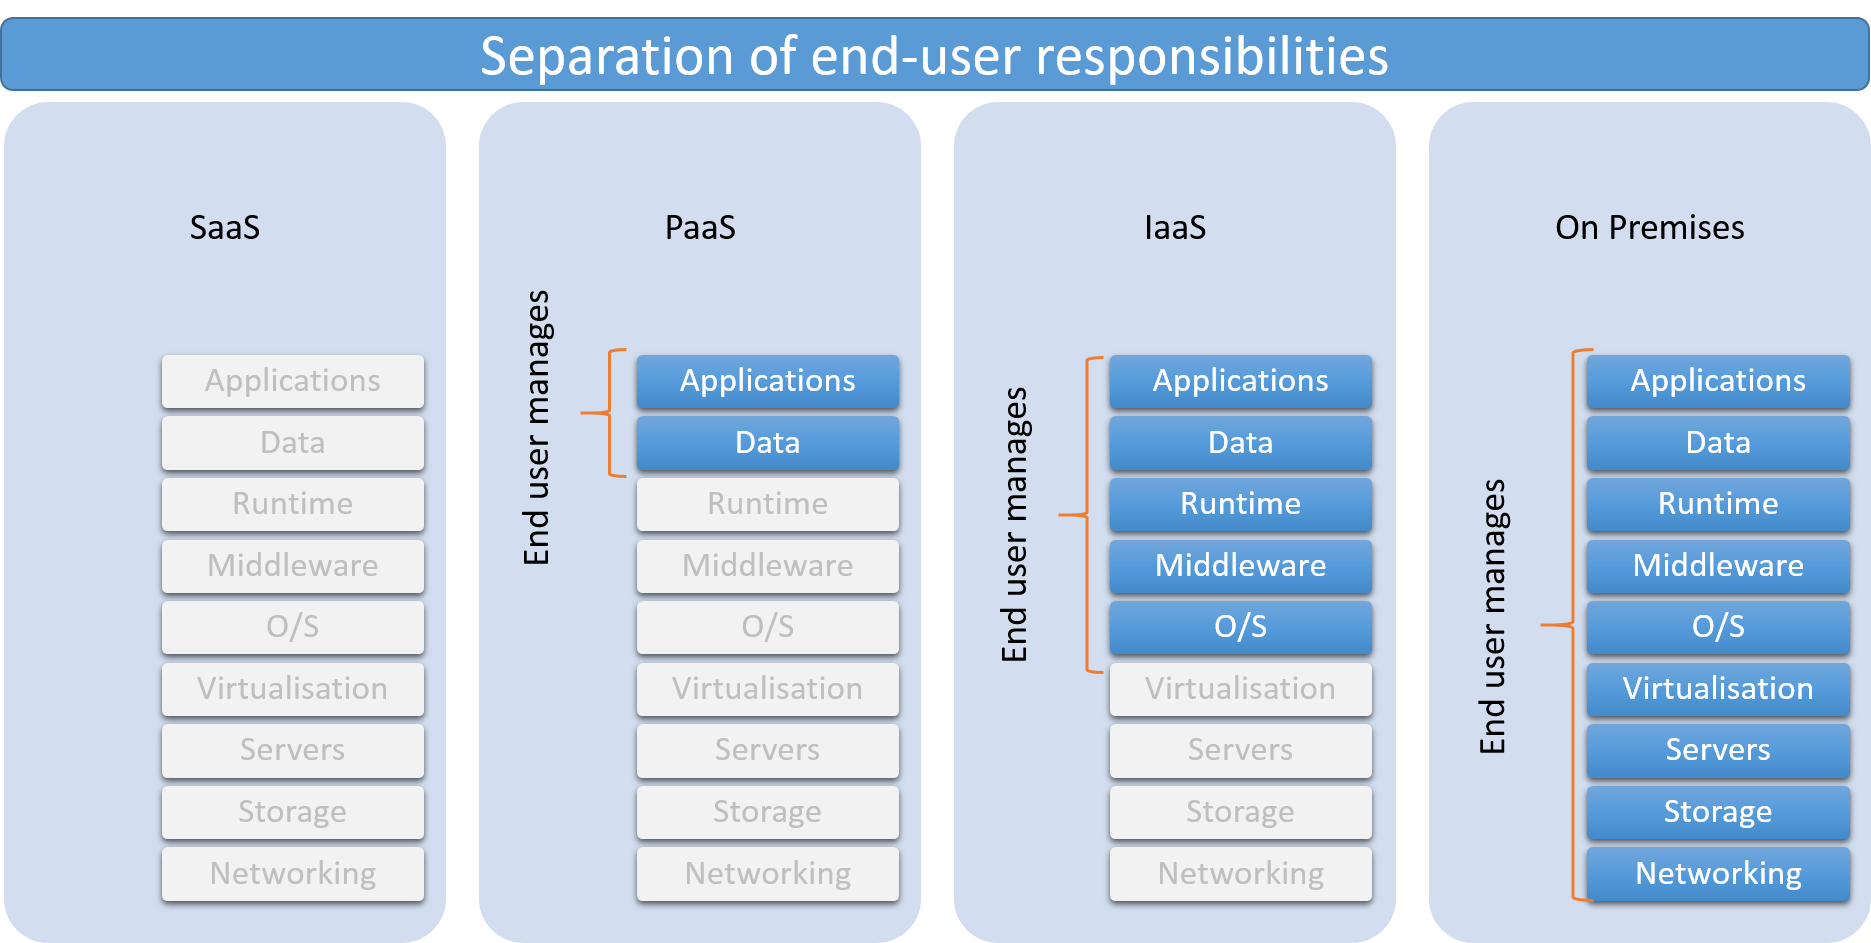
\includegraphics[width=1\linewidth]{responsibilities}
%		\caption{Separation of end user responsibilities based on Internet cloud service model}
%		\label{fig:responsibilities}
%	\end{center}
%	\vspace{-10pt}
%\end{figure}

%The figure \ref{fig:responsibilities} about the cloud service model describes what would be the roles that needs to be played by an end user to utilise and manage each type of service model compared to working on on-premise systems.
%
%\subsection{Software as a Service (SaaS)}\label{ssec:SaaS}
%Software as a service (SaaS) is a software distribution model in which a third-party provider hosts the applications and makes them available to customers over the Internet. Cloud-based applications or software as a service, run on distant computers "in the cloud" that are owned and operated by others and that connect to the user's computer via the Internet and, usually, a web browser.
%
%\begin{figure}[H]
%	\begin{center}
%		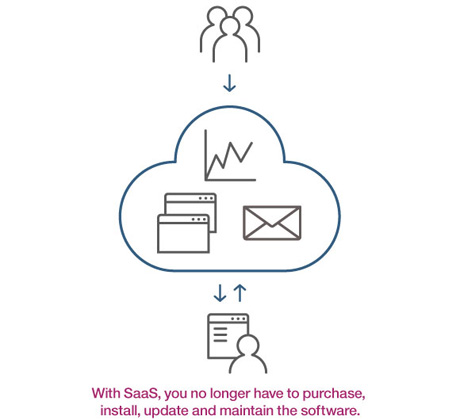
\includegraphics[width=0.95\linewidth]{cc_SaaS}
%		\caption{Software as a service model\cite{IBMcloud:SaaS}}
%		\label{fig:cc_SaaS}
%	\end{center}
%	\vspace{-10pt}
%\end{figure}
%
%SaaS is the most familiar form of cloud service for consumers. SaaS moves the task of managing software and its deployment to third-party services. Among the most familiar SaaS applications for business are customer relationship management applications like Salesforce, productivity software suites like Google Apps, and storage solutions like Box and Dropbox.
%
%Use of SaaS applications tends to reduce the cost of software ownership by removing the need for technical staff to manage the installation, maintenance, and upgrade software, as well as reduce the cost of licensing software. SaaS applications are usually provided on a subscription model.
%
%To summarise the benefits of SaaS:
%\begin{itemize}
%	\item The end user can sign up and rapidly start using innovative business apps
%	\item Apps and data are accessible from any device connected to Internet
%	\item No data is lost if the user's computer or a device breaks, as the data is in the cloud
%	\item The service is able to dynamically scale to the usage needs
%\end{itemize}
%
%\subsection{Platform as a Service (PaaS)}\label{ssec:PaaS}
%Platform as a service (PaaS) is a cloud computing model that delivers development and management tools or applications over the Internet. In a PaaS model, a cloud provider delivers hardware and software tools, "usually those needed for application development", to its users as a service. The provider of the PaaS hosts the hardware and software on their own infrastructure. As a result, PaaS frees the users from having to install in-house hardware and software to develop and run a new application.
%
%It provides a cloud-based environment with everything required to support the complete lifecycle of building and delivering web-based (cloud) applications, without the cost and complexity of buying and managing the underlying hardware, software, provisioning, and hosting. The PaaS provider on request can provide a web development tool or platform which can be customised for the end user.
%
%
%\begin{figure}[H]
%	\begin{center}
%		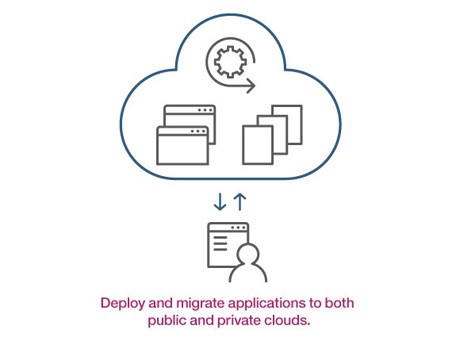
\includegraphics[width=0.95\linewidth]{cc_PaaS}
%		\caption{Platform as a service model\cite{IBMcloud:PaaS}}
%		\label{fig:cc_PaaS}
%	\end{center}
%	\vspace{-10pt}
%\end{figure}
%
%For example, deploying a typical business tool locally might require an IT team to buy and install hardware, operating systems, middleware (such as databases, Web servers and so on) the actual application, define user access or security, and then add the application to existing systems management or application performance monitoring (APM) tools. IT teams must then maintain all of these resources over time. A PaaS provider, however, supports all the underlying computing and software; users only need to log in and start using the platform – usually through a Web browser interface.
%
%Common PaaS vendors include Salesforce.com's Force.com, which provides an enterprise customer relationship management (CRM) platform. PaaS platforms for software development and management include Appear IQ, Mendix, Amazon Web Services (AWS) Elastic Beanstalk, Google App Engine and Heroku.
%
%To summarise the benefits of PaaS:
%\begin{itemize}
%	\item Develop applications and get to market faster
%	\item Deploy new web applications to the cloud in minutes
%	\item Reduce complexity with middleware as a service
%\end{itemize}
%
%\subsection{Infrastructure as a Service (IaaS)}\label{ssec:IaaS}
%
%Infrastructure as a Service (IaaS) is a form of cloud computing that provides virtualized computing resources over the Internet. Infrastructure as a service provides consumers with computing resources including servers, networking, storage, and data center space on a pay-per-use basis.
%
%\begin{figure}[H]
%	\begin{center}
%		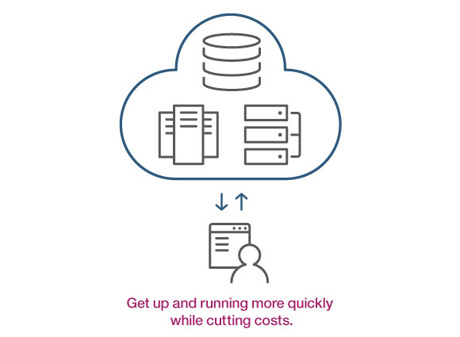
\includegraphics[width=0.95\linewidth]{cc_IaaS}
%		\caption{Infrastructure as a service model\cite{IBMcloud:IaaS}}
%		\label{fig:cc_IaaS}
%	\end{center}
%	\vspace{-10pt}
%\end{figure}
%
%In an IaaS model, a third-party provider hosts hardware, software, servers, storage and other infrastructure components on behalf of its users. IaaS providers also host users' applications and handle tasks including system maintenance, backup and resiliency planning.
%
%IaaS platforms offer highly scalable resources that can be adjusted on-demand. This makes IaaS well-suited for workloads that are temporary, experimental or change unexpectedly.
%
%Other characteristics of IaaS environments include the automation of administrative tasks, dynamic scaling, desktop virtualization and policy-based services.
%
%For example, if a business is developing a new software product, it might be more cost-effective to host and test the application through an IaaS provider. Once the new software is tested and refined, it can be removed from the IaaS environment for a more traditional in-house deployment or to save money or free the resources for other projects.
%
%Leading IaaS providers include Amazon Web Services (AWS), Windows Azure, Google Compute Engine, Rackspace Open Cloud, IBM SmartCloud Enterprise and ProfitBricks.
%To summarise the benefits of IaaS:
%\begin{itemize}
%	\item No need to invest in having or owning the hardware
%	\item Infrastructure scales on demand to support dynamic workloads
%	\item Flexible, innovative services available on demand
%\end{itemize}

%\section{Summary about "The Cloud"}\label{sec:intro1_summary}
%The cloud has become a key enabler for today's small or medium sized business to unlock creativity, drive unrivaled innovation and level the competition with larger enterprise competitors.
%
%Prior to the advent of cloud-based products software solutions delivered over the Internet companies were often forced to invest in servers and other products to run software and store data. The advent of cloud services as well as their steady improvement in such areas as security and reliability make these solutions a logical choice for business owners and principals who want the latest innovations, functionality, and efficiency as well as cost effectiveness.
%
%Many businesses garner considerable cost savings by migrating their software systems to the cloud. In addition to reducing reliance on the purchase and maintenance of servers, companies often lower their information technology costs in such areas as dedicated personnel and software upgrades. Most cloud services upgrade and update software via the Internet with little or no downtime for end users, decreasing the wait time associated with installing and testing software on an on-site network. Moreover, cloud-based products are scalable: unlike conventional software, cloud services can be expanded as needed to encompass as many end users as required without additional overhead of servers and upgrades to handle added workloads.
%
%When more number of small and medium sized business begin to realize that the cloud can do more than just reduce the cost of IT, the journey to the cloud becomes inevitable and the question shifts from whether to adopt cloud technologies to how to do so sensibly.
%
%It is fascinating to understand the working of cloud as it has created lot of new opportunities for research, jobs and investment in this domain.